\documentclass[12pt,AutoFakeBold]{article} 

\usepackage[智能数据挖掘]{XDUreport}  % 科目名称
\problem{UCI Musk 数据集特征提取分析报告}  % 请在此处填写问题内容
% 其他参数在宏包中进行更改,其中学院,班级,姓名,学号均在sty宏包内进行更改
% \usepackage{fourier}  % 这是 fourier 字体,更柔和 

%% 如果你需要中文的一级标题编号,如“一、”、“二、”等,请把下面两行取消注释
% \RequirePackage{zhnumber} % change section number to chinese
% \titleformat{\section}{\Large\bfseries\rmfamily}{\zhnum{section}、}{0em}{}

% 文档开始
        
\begin{document}

\maketitle
\setcounter{tocdepth}{2}

\tableofcontents  % 生成目录

% 正文标题
\makeatletter
\begin{center}
    \LARGE \textbf{\textsf{\@problem}}
\end{center}
\makeatother

% 正文开始

\section{Musk 数据集简介}

Musk (麝香) 数据集 (版本 1) 有 476 行 169 列,共 166 个属性 2 类标签。该数据集描述了一组 92 个分子,其中 47 个被人类专家判断为麝香,其余 45 个分子被判断为非麝香。目标是学习预测新分子是麝香还是非麝香。然而,描述这些分子的 166 个特征取决于分子的确切形状或构象。因为键可以旋转,单个分子可以采用许多不同的形状。为了生成这个数据集,生成了分子的低能构象,然后过滤以去除高度相似的构象。这留下了 476 个构象。然后,提取描述每个构象的特征向量。

特征向量和分子之间的这种多对一关系称为“多实例问题”。在为该数据学习分类器时,如果分子的任何构象被分类为麝香,分类器应将其分类为“麝香”。如果分子的构象中没有一个被归类为麝香,则该分子应归类为“非麝香”。各列说明如下:

\begin{itemize}
\item 	
molecule\_name (列 1):每个分子的符号名称。麝香有诸如 MUSK-188 之类的名称。非麝香具有诸如 NON-MUSK-jp13 之类的名称。
\item onformation\_name (列 2):每个构象的符号名称。它们的格式为 MOL\_ISO+CONF,其中 MOL 是分子编号,ISO 是立体异构体编号(通常为 1),CONF 是构象编号。
\item f1 到 f162:这些是沿射线的“距离特征”。距离以百分之几埃为单位。距离可以是负数或正数,因为它们实际上是相对于沿每条射线放置的原点测量的。起源由不再使用的“共识麝香”表面定义。因此,任何对数据的实验都应将这些特征值视为位于任意连续尺度上。特别是,算法不应使用零点或每个特征值的符号。
\item f163:这是分子中的氧原子到 3 空间中指定点的距离。这也称为 OXY-DIS。
\item f164:OXY-X:从指定点开始的 X 位移。
\item f165:OXY-Y:从指定点开始的 Y 轴位移。
\item f166:OXY-Z:从指定点开始的 Z 位移。
\item class: 0 $\Rightarrow$ non-musk, 1 $\Rightarrow$ musk。
\end{itemize}

\section{原理分析}

\subsection{数理统计知识}

设随机变量 $X$ 期望为 $\mathrm{E}[X]=\mu$,计算方差如下
%
\begin{equation}
\mathrm{Var}(X)=\sigma^2=E[(X-\mu)^2]
\end{equation}
%
上式计算需要知道 $X$ 具体分布,实际采样用 $S^2$ 近似 $\sigma^2$
%
\begin{equation}
S^2=\frac{1}{n}\sum_{i=1}^n\left(X_i-\mu\right)^2
\end{equation}
%
但现实中往往 $\mu$ 也不清楚,只知道样本均值 $\overline{X}=\frac{1}{n}\sum_{i=1}^nX_i$,总体样本估计值为
%
\begin{equation}
\sigma_X^2=\frac{1}{n}\sum_{i=1}^n\left(X_i-\overline{X}\right)^2
\end{equation}
%
利用结论 $\mathrm{Var}(X)=\mathrm{E}[X^2]-\mathrm{E}[X]^2$,计算期望如下
%
\begin{equation}
\begin{aligned}
\mathrm{E}[\sigma_X^2] &= \mathrm{E}\left[\frac{1}{n}\sum_{i=1}^n\left(X_i-\overline{X}\right)^2\right] \\
 &= \frac{1}{n}\sum_{i=1}^n\mathrm{E}\left[X_i^2-\frac{2}{n}X_i\sum_{j=1}^nX_j+\frac{1}{n^2}\sum_{j=1}^nX_j\sum_{k=1}^nX_k\right] \\
 &= \frac{1}{n}\sum_{i=1}^{n}\left(\frac{n-2}{n}\mathrm{E}[X_i^2]-\frac{2}{n}\sum_{j\neq i}\mathrm{E}[X_iX_j]+\frac{1}{n^2}\sum_{j=1}^n\sum_{k\neq j}E[X_jX_k]+\frac{1}{n^2}\sum_{j=1}^nE[X_j^2]\right) \\
 &= \frac{1}{n}\sum_{i=1}^{n}\left[\frac{n-2}{n}(\sigma^2+\mu^2)-\frac{2}{n}(n-1)\mu^2+\frac{1}{n^2}n(n-1)\mu^2+\frac{1}{n}(\sigma^2+\mu^2)\right] \\
 &= \frac{n-1}{n}\sigma^2
\end{aligned}
\end{equation}
%
为了避免偏差,采用修正值
%
\begin{equation}
S^2=\frac{1}{n-1}\sum_{i=1}^n\left(X_i-\overline{X}\right)^2
\end{equation}
%

\subsection{特征值分解}

\subsubsection{特征值与特征向量}

若向量 $v$ 是矩阵 $\bm{A}$ 的特征向量,一定可以表示成如下的形式:
%
\begin{equation}
\bm{A}v=\lambda v\Rightarrow (\lambda \bm{E}-\bm{A})v=0
\end{equation}
%
其中,$\lambda$ 是特征向量 $v$ 对应的特征值,矩阵的一组特征向量是一组正交向量。

\subsubsection{特征值分解}

对于矩阵 $\bm{A}$,有一组特征向量 $v$,将这组向量进行正交化单位化,就能得到一组正交单位向量。特征值分解,就是将矩阵 $\bm{A}$ 分解为如下式:
%
\begin{equation}
\bm{A}=Q\Lambda Q^{-1}
\end{equation}
%
其中,$Q$ 是矩阵 $\bm{A}$ 的特征向量组成的矩阵,$\Lambda$ 是对角阵,对角线上的元素就是特征值。

\subsection{PCA 降维}

主成分分析 (Principal components analysis,PCA) 是一种常用的降维方法,主要思想是将 $n$ 维特征映射到 $k$ 维上,$k$ 维正交新特征被称为主成分。PCA 在原始空间中找一组相互正交的坐标轴,其中,第一个新坐标轴选择是原始数据中方差最大的方向,第二个新坐标轴选取是与第一个坐标轴正交的平面中使得方差最大的,第三个轴是与第 $1,2$ 个轴正交的平面中方差最大的,以此类推得到 $n$ 个这样的坐标轴,部分方差都包含在前面 $k$ 个坐标轴中,后面的坐标轴所含的方差几乎为 $0$,故可以忽略余下的坐标轴,只保留前面 $k$ 个含有绝大部分方差的坐标轴,实现对数据特征的降维处理。

\begin{algorithm}[hbtp]
	\caption{PCA 算法} \label{PCA}
	\begin{algorithmic}[1]
	\Require 样本集 $D=\{\bm{x}_1,\bm{x}_2,\cdots,\bm{x}_n\}$,低维空间维数 $k$
	\Ensure 投影矩阵 $P$ 和新空间中的数据表示
	\State 所有样本中心化: $\bm{x}_i\leftarrow \bm{x}_i-\frac{1}{n}\sum_{i=1}^n\bm{x}_i$
	\State 计算样本协方差矩阵 $\frac{1}{n}XX^T$
	\State 对协方差矩阵 $\frac{1}{n}XX^T$ 做特征值分解得到特征值与特征向量
	\State 特征值从大到小排序,取最大的 $k$ 个,对应的 $k$ 个特征向量作为行向量组成投影矩阵 $P$
	\State 将数据据转换到新空间中 $Y=PX$
	\end{algorithmic}
\end{algorithm}

\subsection{SVD 降维}

奇异值分解 (Singular value decomposition,SVD) 是线性代数中一种重要的矩阵分解,适用于任意矩阵。对于任意矩阵 $\bm{A}$ 总是存在一个奇异值分解:
%
\begin{equation}
\bm{A}=\bm{U}\Sigma \bm{V}^T
\end{equation}
%
假设 $\bm{A}$ 是一个 $m\times n$ 阶矩阵,那么得到的 $\bm{U}$ 是一个 $m\times m$ 阶方阵,$\bm{U}$ 里面的正交向量被称为左奇异向量。$\Sigma$ 是一个 $m\times n$ 阶矩阵,$\Sigma$ 除了对角线其它元素都为 0,对角线上的元素称为奇异值。 $\bm{V}$ 是 $\bm{V}$ 的转置矩阵,是一个 $n\times n$ 阶矩阵,它里面的正交向量被称为右奇异值向量。一般而言,我们将 $\Sigma$ 上的值按从大到小的顺序排列。对矩阵 $\bm{A}$ 进行 SVD 分解的步骤如下:

\begin{enumerate}
\renewcommand{\labelenumi}{\hspace{12pt} \bfseries \textit{Step} \theenumi.}

\item 计算 $\bm{A}\bm{A}^T$ 的特征值和特征向量,用单位化的特征向量构成 $\bm{U}$。

\item 计算 $\bm{A}^T\bm{A}$ 的特征值和特征向量,用单位化的特征向量构成 $\bm{V}$。

\item 计算 $\bm{A}\bm{A}^T$(or $\bm{A}^T\bm{A}$) 的特征值求平方根,然后构成 $\Sigma$。
\end{enumerate}

经过 SVD 分解后,可以用前 $k$ 个非零奇异值对应的奇异向量表示矩阵 $A$ 的主要特征,这样就把矩阵 $A$ 进行了降维。

\section{实验过程}

\subsection{PCA 降维}

导入数据集和预处理后,为了合理选择主成分个数,我利用特征值分解的 PCA 对主成分的贡献率和贡献增长率进行分析,如图 \ref{fig:contributions} 所示,红色曲线表示总贡献率,蓝色曲线表示贡献增长率,可见 10 个主成分后贡献增长率接近于 0,且 10 个主成分共享率为 83\%,故可选择 10 个主成分进行后续实验。

\begin{figure}[htbp]
	\centering
    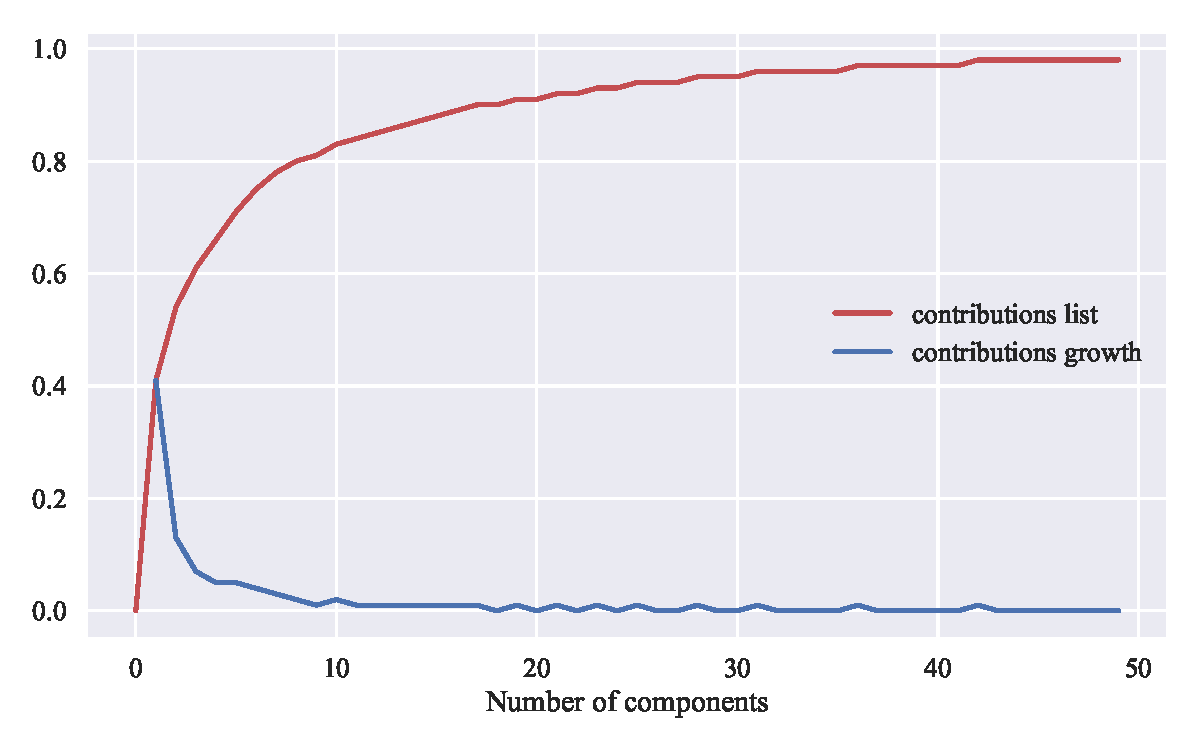
\includegraphics[width=0.7\textwidth]{contributions.pdf}
    \caption{主成分贡献率和贡献增长率曲线} \label{fig:contributions}
\end{figure}

\begin{figure}[htbp]
	\centering
    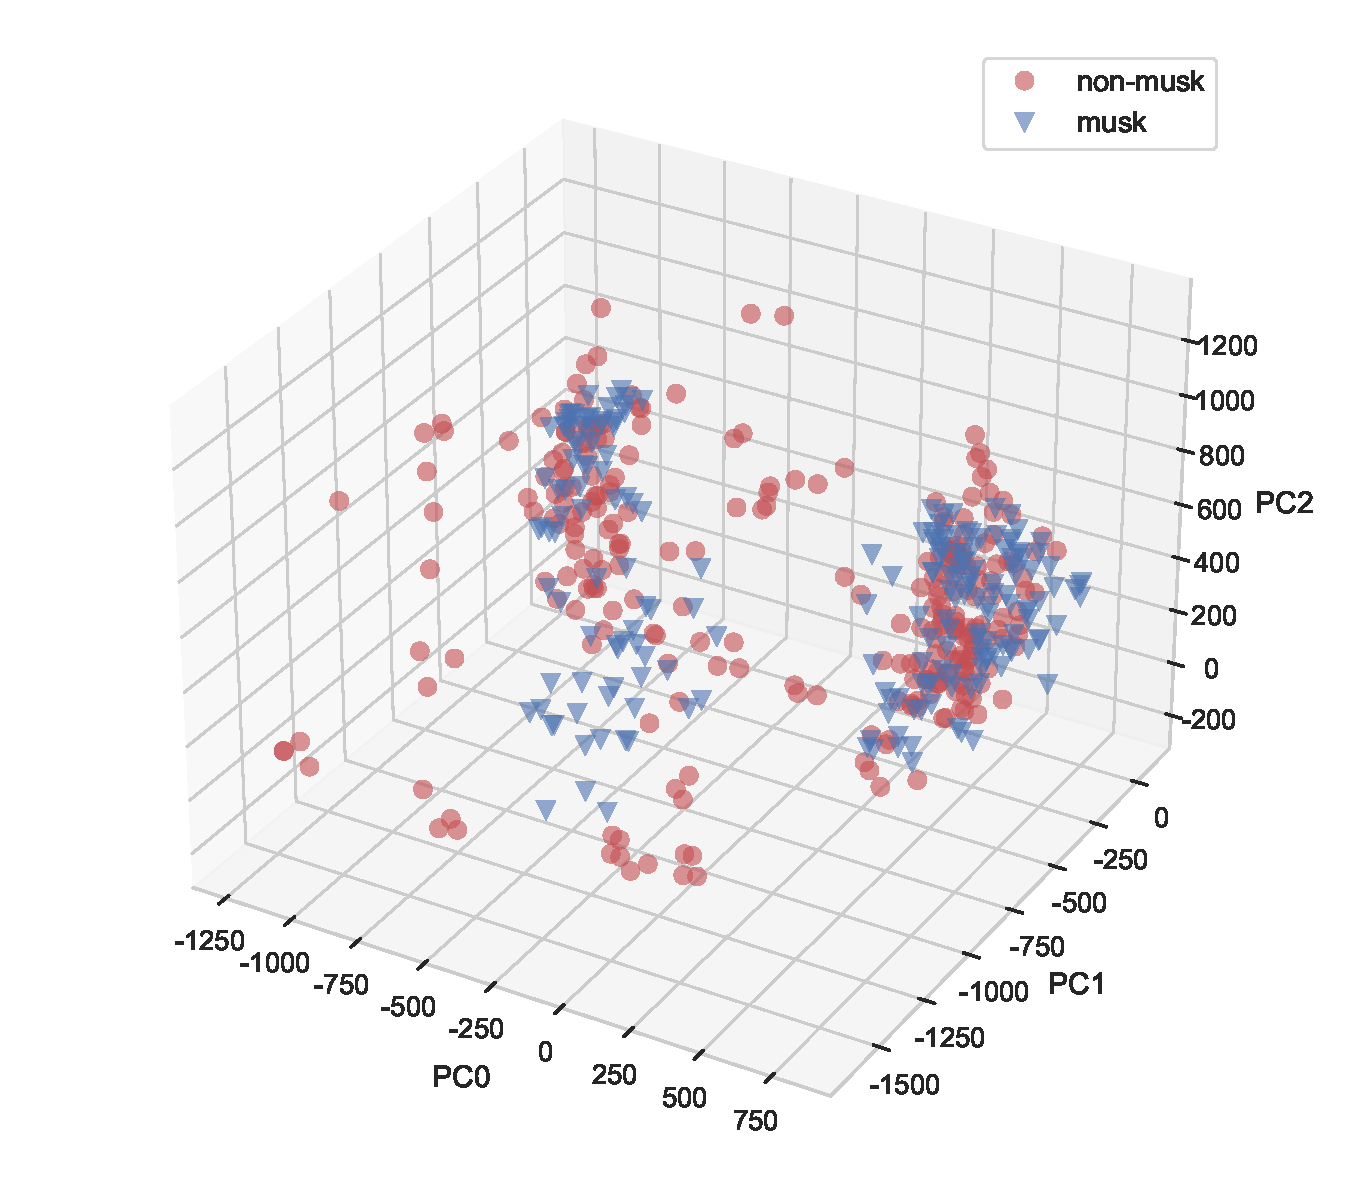
\includegraphics[width=0.7\textwidth]{plot_3D.pdf}
    \caption{前 3 个主成分散点图} \label{fig:plot_3D}
\end{figure}

10 个主成分降维获得的特征值为 $[453240\ 144754\ 77811\ 62336\ 49078\ 46722\ 30678\ 23609\ \allowbreak 18173\ 17244]$,由于特征向量和降维后的数据太长,具体结果见附录后的代码和结果。之后取前 3 个主成分绘制散点图进行可视化观察分析,如图 \ref{fig:plot_3D} 所示,由之前分析知前三个主成分只有不到 50\% 贡献率,故不能很好分类。

现在绘制获得新数据的盒图 (boxplot),一个盒图的示例如图 \ref{fig:boxplot1} 所示,可以告诉我们异常值有哪些、数据是否对称、数据分组的紧密程度以及数据是否和怎样倾斜。它由五个数值点组成:最小值 (min),下四分位数 (Q1),中位数 (median),上四分位数 (Q3),最大值 (max)。也可以往盒图里面加入平均值 (mean)。

\begin{figure}[htbp]
	\centering
    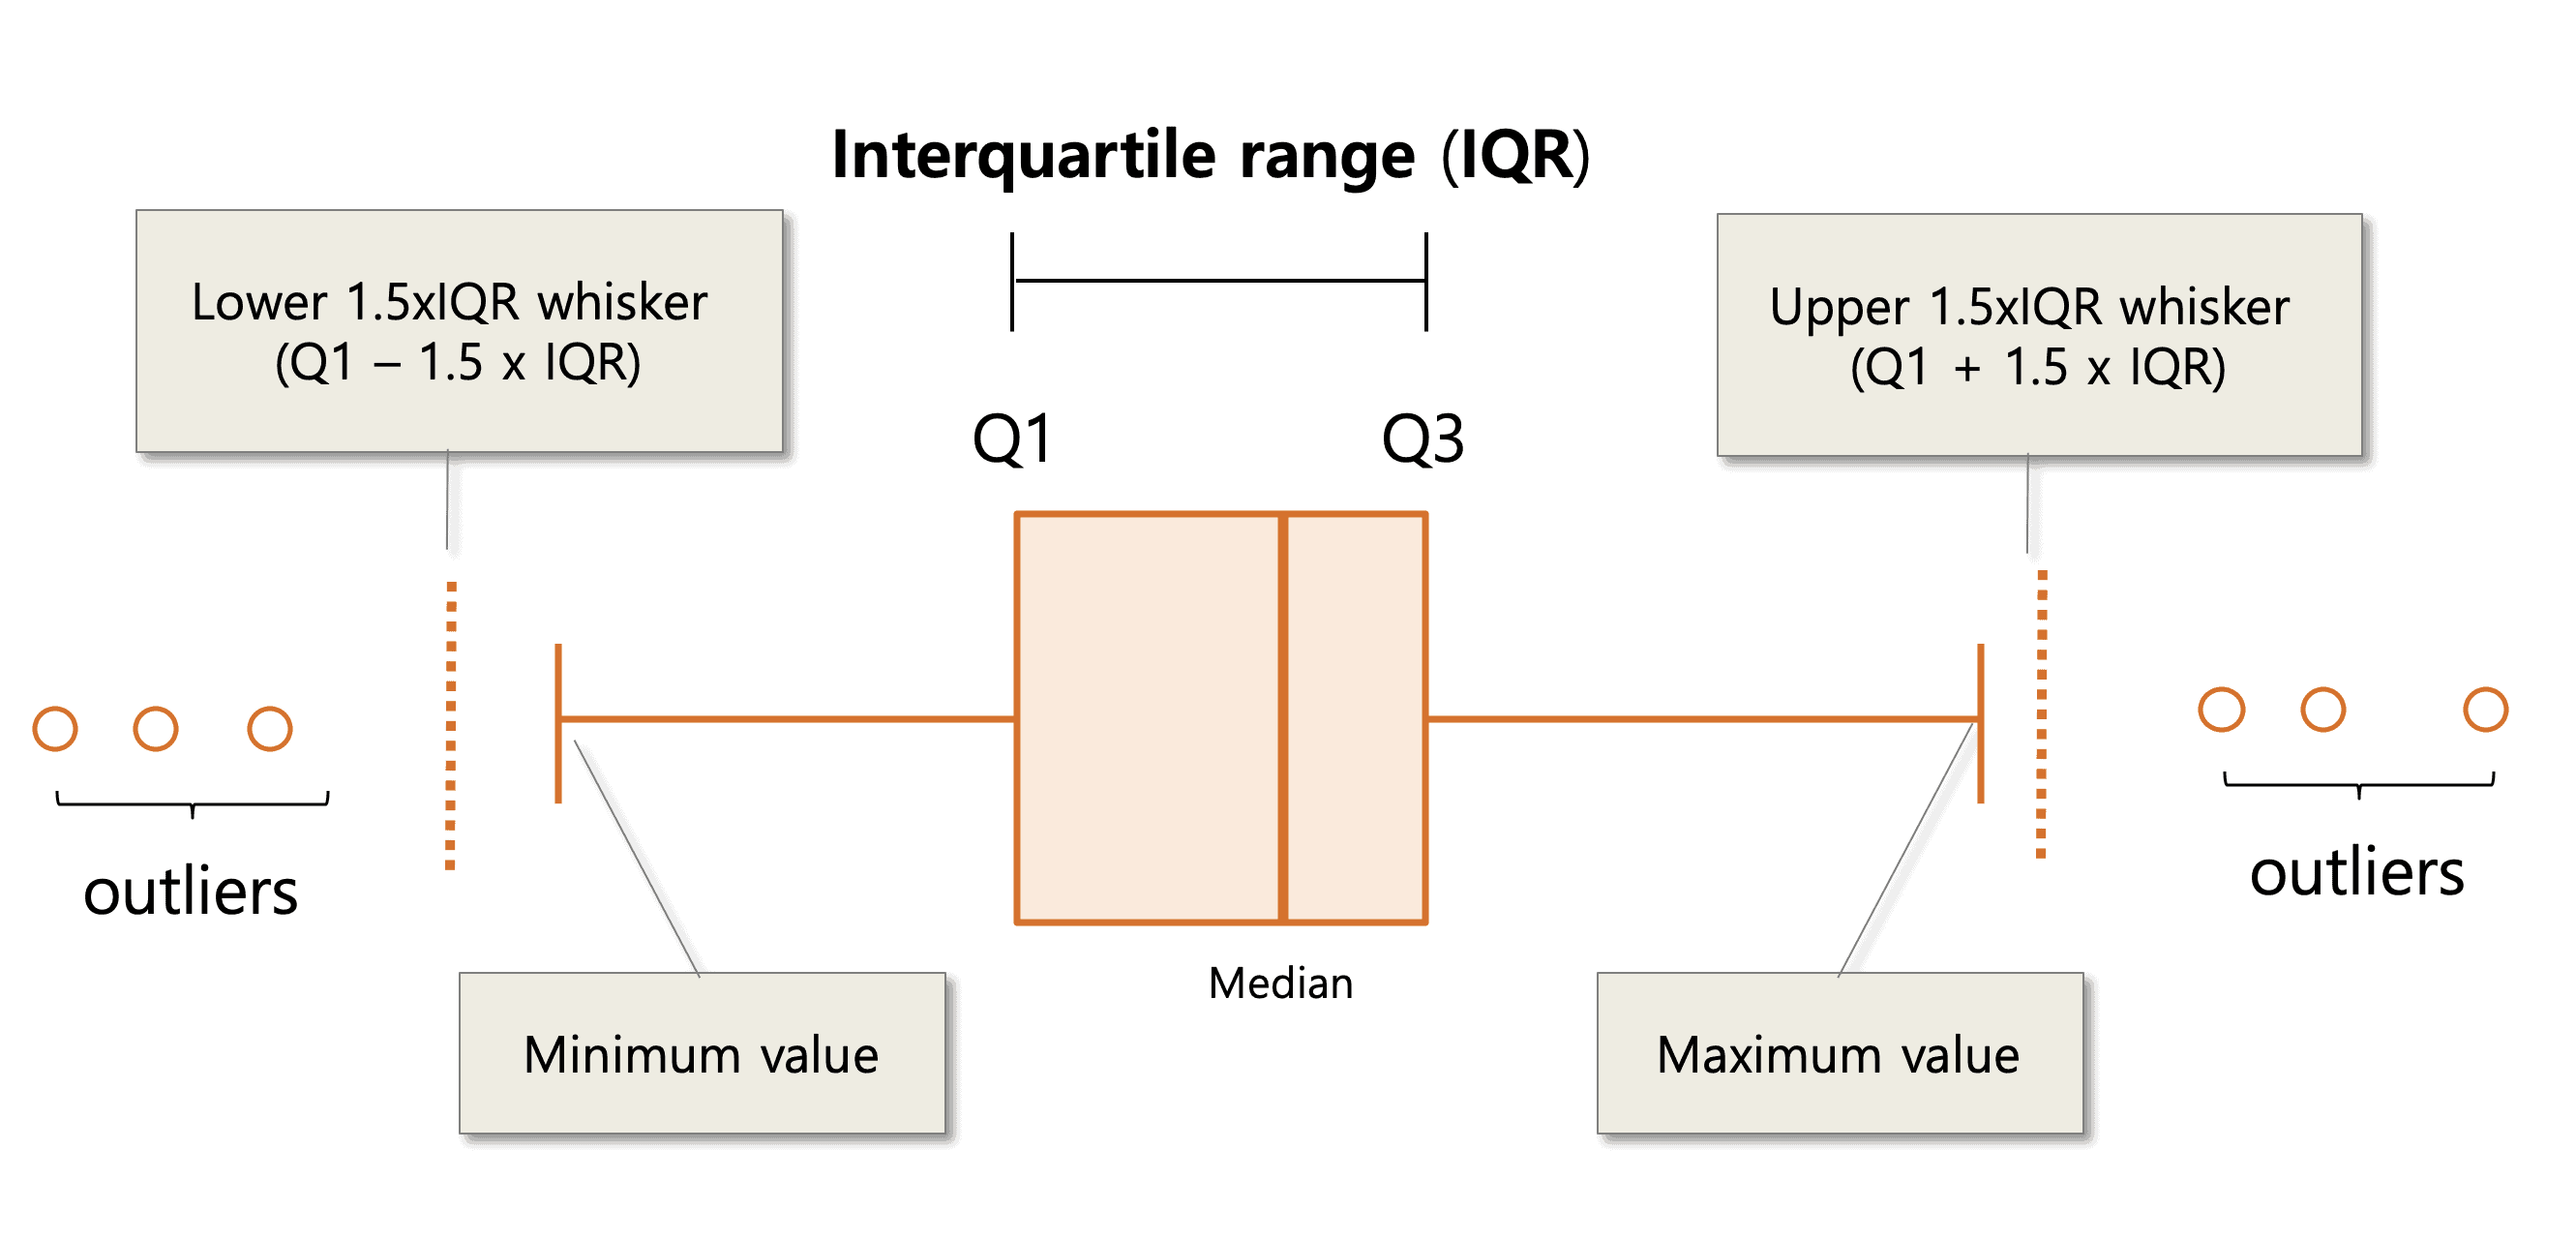
\includegraphics[width=0.7\textwidth]{boxplot1.png}
    \caption{盒图示例} \label{fig:boxplot1}
\end{figure}

利用 PCA 降维获得的新数据绘制的盒图如图 \ref{fig:boxplot_pca} 所示,绿色虚线表示平均值。

\begin{figure}[htbp]
	\centering
    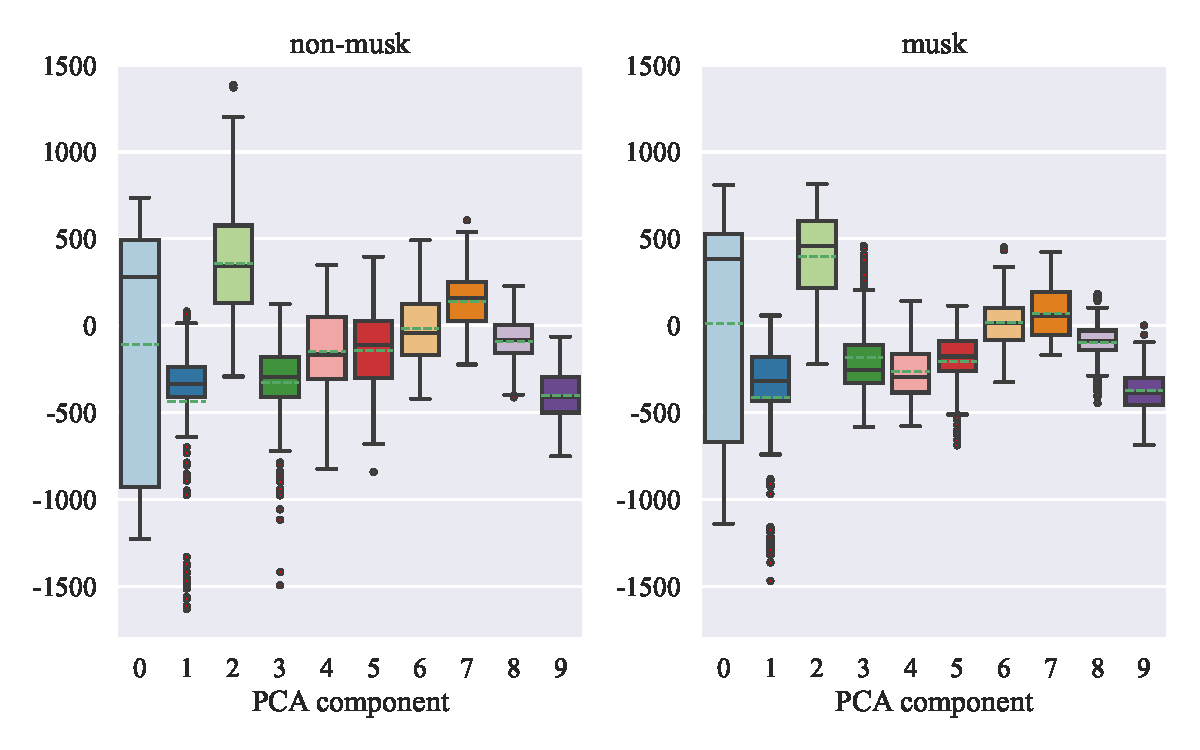
\includegraphics[width=\textwidth]{boxplot_pca.pdf}
    \caption{PCA 降维后新数据盒图} \label{fig:boxplot_pca}
\end{figure}

\subsection{SVD 降维}

取 $k$ 个奇异值使得占总奇异值的 90\%,可以进行压缩存储,计算得 $k=18$。利用 SVD 降维获得的新数据绘制的盒图如图 \ref{fig:boxplot_svd} 所示,绿色虚线表示平均值。

\begin{figure}[htbp]
	\centering
    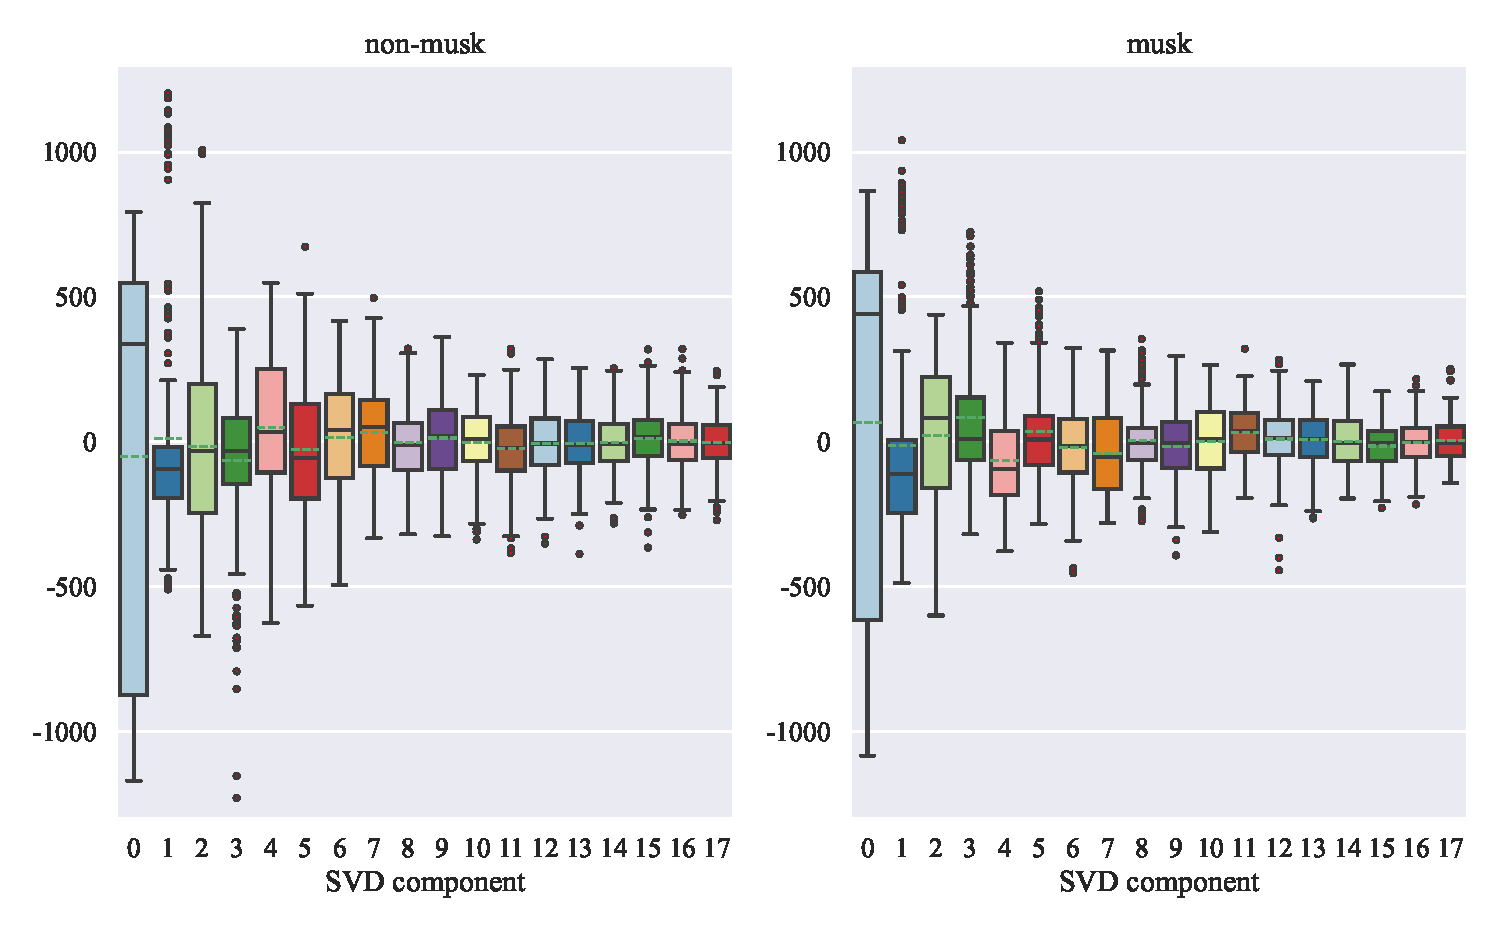
\includegraphics[width=\textwidth]{boxplot_svd.pdf}
    \caption{SVD 降维后新数据盒图} \label{fig:boxplot_svd}
\end{figure}

\section{总结}

通过此次实验,我回顾了数理统计中样本方差以及 PCA、SVD 降维的相关知识,掌握了盒图的概念和 Python 中盒图的画法。具体 Jupyter Notebook 代码和结果见附录。

\includepdfset{pagecommand={\thispagestyle{fancy}}} 
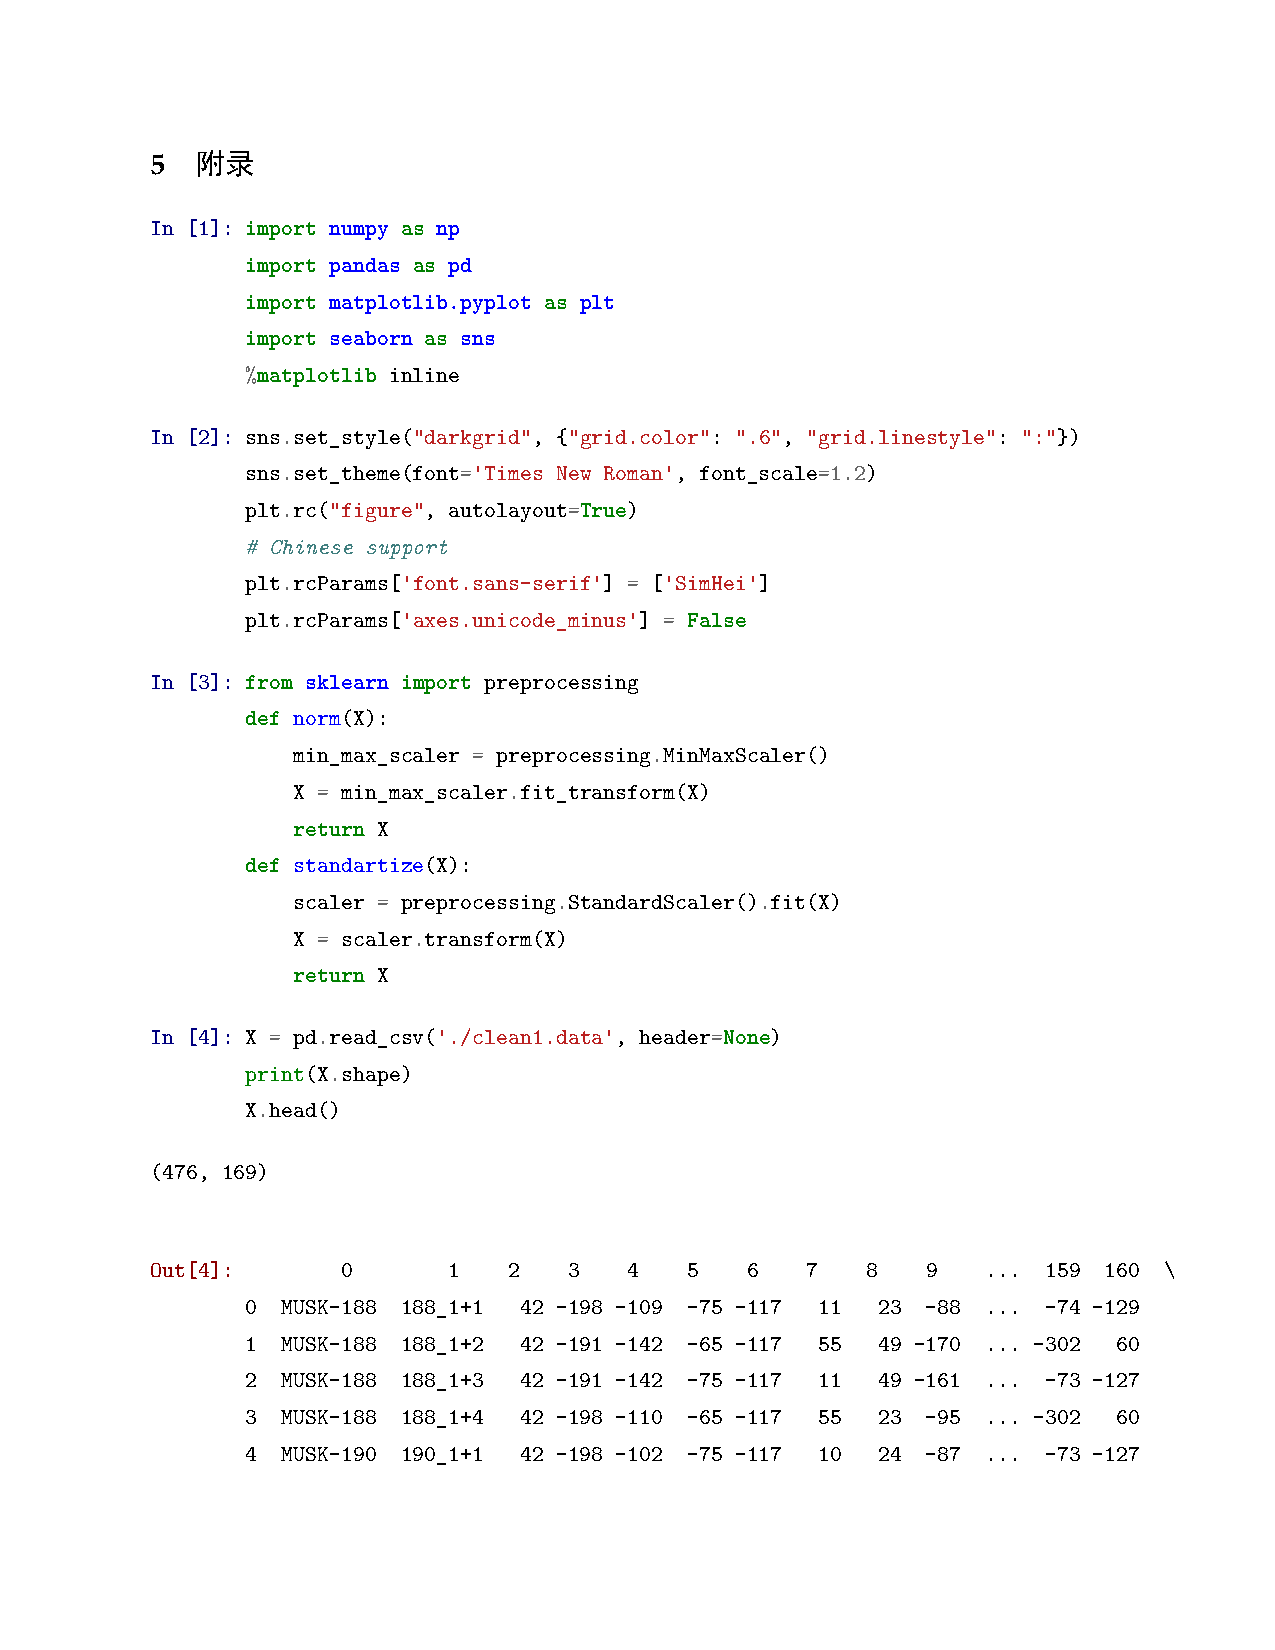
\includepdf[addtotoc={1,section,1,附录,appendix}, pages={1-11}]{PCA_SVD.pdf}

% % 参考文献,此处以 MLA 引用格式为例

% \begin{thebibliography}{9}
%     \bibitem{1} Clemente, Filipe Manuel, et al. "General network analysis of national soccer teams in FIFA World Cup 2014." \emph{International Journal of Performance Analysis in Sport} 15.1 (2015): 80-96.
%     \bibitem{3} Dijkstra, Edsger Wybe. "A Note on Two Problems in Connexion With Graphs." \emph{Numerische Mathematik} 1(1959):269-271.
%     \bibitem{4} Ahnert, Sebastian E., et al. "Ensemble approach to the analysis of weighted networks.." \emph{Physical Review E} 76.1 (2007).
%     \bibitem{5} Wong, J. A. Hartiganm. A. . "Algorithm AS 136: A K-Means Clustering Algorithm." \emph{Journal of the Royal Statistical Society. Series C (Applied Statistics)} 28.1(1979):100-108.
%     \bibitem{6} Buldu, J. M., et al. "Defining a historic football team: Using Network Science to analyze Guardiola’s F.C. Barcelona." \emph{Scientific Reports} 9.1 (2019): 1-14.
%     \bibitem{7} \emph{Balotelli sends Italy past Germany}. (2012). Retrieved December 10, 2014, from\url{https://www.uefa.com/uefaeuro/season=2012/matches/round=15174/match=2003379/index.html}
%     \bibitem{8} Sigari, Mohamad Hoseyn, et al. "Counterattack detection in broadcast soccer videos using camera motion estimation." \emph{international symposium on artificial intelligence} (2015): 101-106.
%     \bibitem{9} Abdelmahmoud Hassan Elsheikh. \emph{Effect of Leadership Intensity on Integrating Some Formal and Informal Organizational Efforts for Community Development in Khartoum Province}. 2016.
% \end{thebibliography}


% \includepdf[pages={1,2}]{Memo.pdf} 
% 可以直接导入pdf页面
% \newpage
% \begin{appendices}  % 附录环境
% \section{附录}
% \end{appendices}

\end{document}  % 结束